\documentclass{beamer}
\title{Customer Churn Prediction}
\author{Analyst}

\usepackage{graphicx}

\begin{document}

% Title Slide
\begin{frame}
    \titlepage
\end{frame}

% Motivation Slide
\begin{frame}{Motivation}
    Churn is a significant challenge, affecting revenue and growth. \\ The goal of this project is to predict which customers may churn and identify the key factors influencing this process.
\end{frame}

% Problem Statement Slide
\begin{frame}{Problem Statement}
    The need to accurately forecast customer churn to minimize losses and improve customer retention.
\end{frame}

% Methodology Slide
\begin{frame}{Methodology}
    \begin{itemize}
        \item Data includes demographics, transaction history, service usage, and customer support interactions.
        \item Machine learning algorithms used: Logistic Regression, Random Forest, Gradient Boosting (XGBoost).
    \end{itemize}
\end{frame}

% Solution Slide
\begin{frame}{Solution}
    Developed a model to predict customer churn effectively based on historical data. \\ Advanced machine learning algorithms improve prediction accuracy and identify key risk factors.
\end{frame}

% Key Steps Slide
\begin{frame}{Key Steps}
    \begin{enumerate}
        \item \textbf{Data Collection and Preparation}: Cleaning and processing customer data.
        \item \textbf{Modeling}: Logistic regression as a baseline, then exploring Random Forest and Gradient Boosting.
        \item \textbf{Model Evaluation}: Metrics such as accuracy, F1 score, and ROC-AUC are used to assess the model's performance.
    \end{enumerate}
\end{frame}

% Graphical Results Slide
\begin{frame}{Graphical Results}
    \begin{itemize}
        \item \textbf{ROC Curve}: Shows the balance between true positives and false positives.
        \begin{figure}[h]
            \centering
            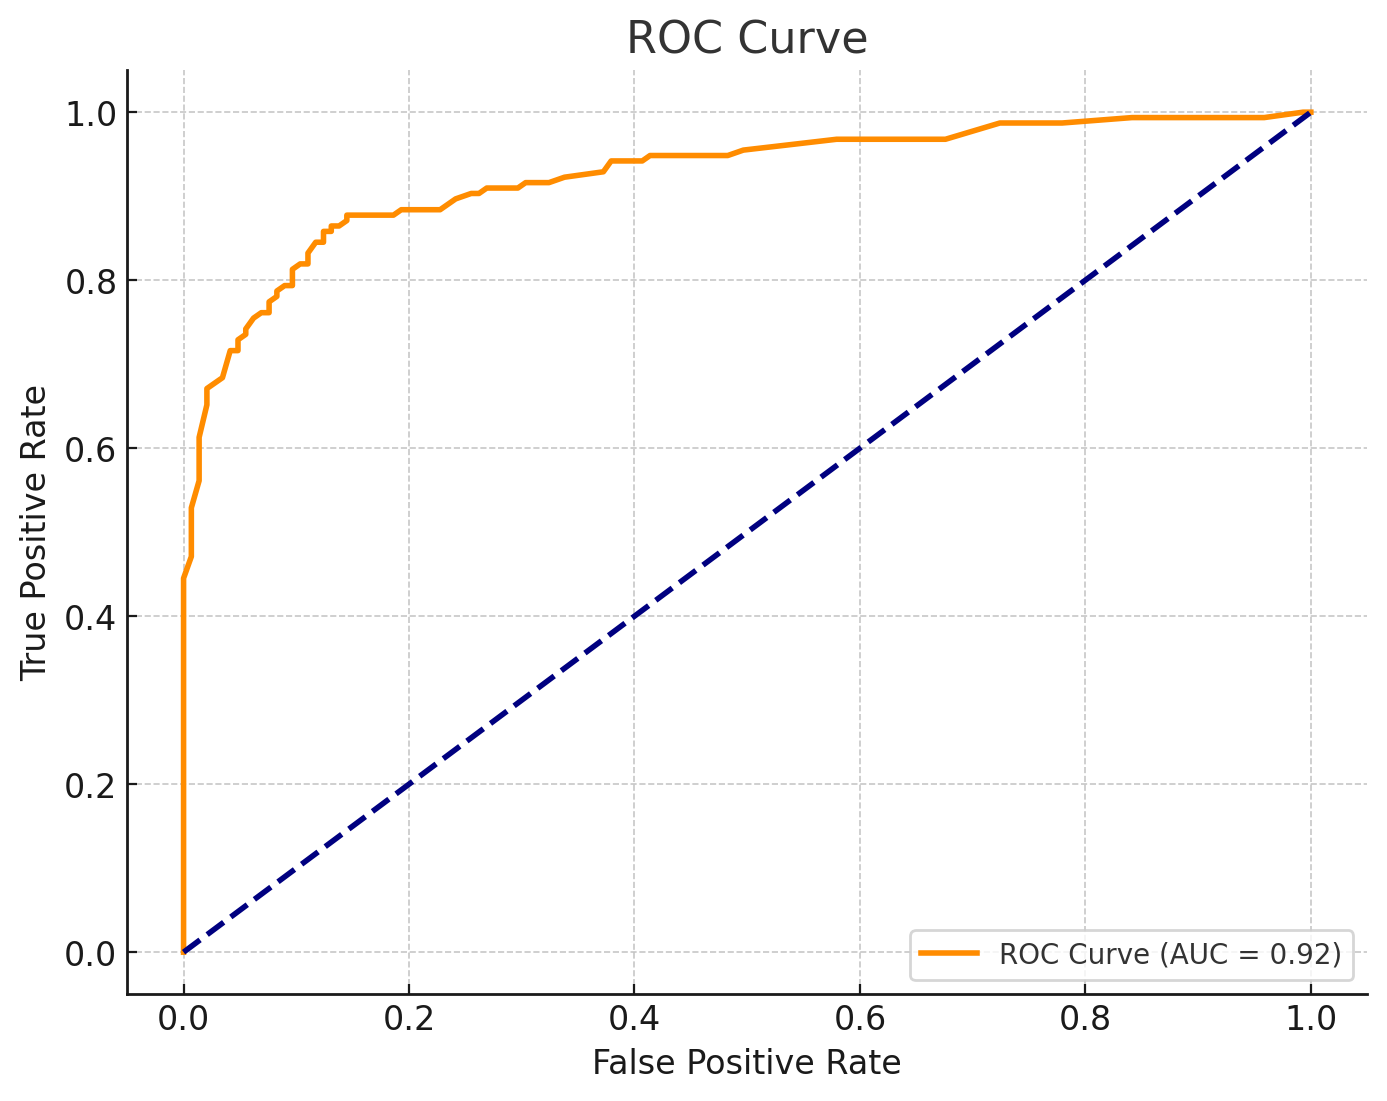
\includegraphics[width=0.8\linewidth]{Shirshov-Step-3-fig.png}
            \caption{ROC Curve}
        \end{figure}
    \end{itemize}
\end{frame}

% Impact Slide
\begin{frame}{Impact}
    The findings will help marketing and customer success teams allocate resources more effectively, improving retention and customer lifetime value.
\end{frame}

% Conclusion Slide
\begin{frame}{Conclusion}
    The model provides a practical tool for predicting customer churn, with the potential to optimize retention strategies. \\ Regular updates are necessary to maintain accuracy as customer behavior evolves.
\end{frame}

\end{document}
